\itemhead{p.72 练习 · 第3题（教材p.72）}{XJ-B1-C03-PR-P072-Y1416}
\label{XJ-B1-C03-PR-P072-Y1416}
{\footnotesize 湘教版教材p.72 / PDF第79页 / p.72 练习 / 第3题}
\field{原题}{画出函数 $f(x)=-x^2+2x+3$ 的图象，并根据图象回答下列问题：
\subq{1}比较 $f(0),f(1),f(3)$ 的大小；
\subq{2}若 $x_1<x_2<1$，比较 $f(x_1)$ 与 $f(x_2)$ 的大小；
\subq{3}求函数 $f(x)$ 的值域。}
\field{参考答案}{$f(x)=-(x-1)^2+4$，顶点 $(1,4)$，与 $x$ 轴交于 $(-1,0),(3,0)$。（1）$f(3)=0<f(0)=3<f(1)=4$；（2）$f(x_1)<f(x_2)$；（3）值域 $(-\infty,4]$。}
\begin{center}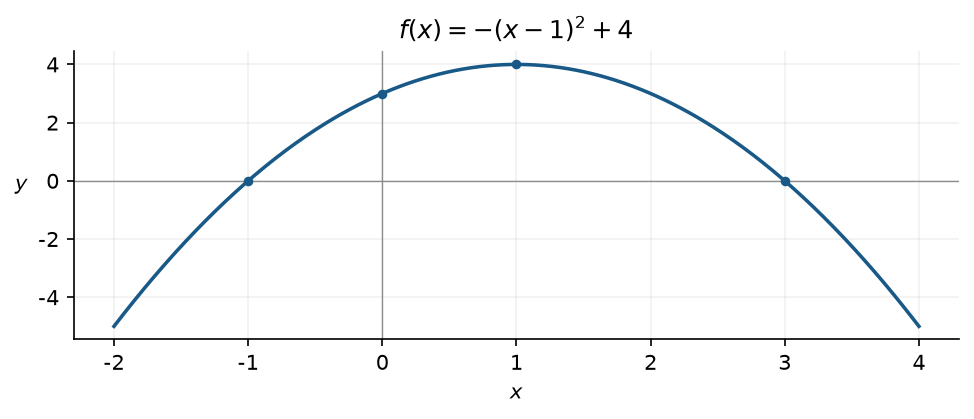
\includegraphics[width=.84\linewidth,height=.38\textheight,keepaspectratio]{figures/C03-PR072-3.png}\end{center}
\field{核对说明}{答案册方向笔误：答案册PDF19第3题第2问写f(x1)>f(x2)；在x1<x2<1时二次函数递增，正确为f(x1)<f(x2)。}
{\small \field{关联知识}{F04 函数三种表示法、图象与读数（教材帮p.85、86、93、94 / PDF94、95、102、103）；F05 单调性定义、证明与参数（教材帮p.97、98、100 / PDF106、107、109）；F06 最大值、最小值与值域（教材帮p.99、83、84 / PDF108、92、93）}
\field{方法与易错点}{把关键点与定义域一起标到图上，逐区间读交点和上下关系。 易错：将示意图预测当事实；把两曲线交点收进严格不等式；折线漏端点。}
\field{答案依据}{答案册相关题组：PDF第19页（册内页18）；按当前题库原题逐项重算，不按旧版题号机械对套。}}
